\documentclass[11pt]{amsart}
\usepackage{geometry}                % See geometry.pdf to learn the layout options. There are lots.
\geometry{letterpaper}                   % ... or a4paper or a5paper or ...
%\geometry{landscape}                % Activate for for rotated page geometry
%\usepackage[parfill]{parskip}    % Activate to begin paragraphs with an empty line rather than an indent
\usepackage{graphicx}
\usepackage{amssymb}
\usepackage{epstopdf}
\usepackage[usenames,dvipsnames]{color}
\usepackage{hyperref}
\usepackage{subfig}
\usepackage{float}
\hypersetup{colorlinks=true}
\DeclareGraphicsRule{.tif}{png}{.png}{`convert #1 `dirname #1`/`basename #1 .tif`.png}
\renewcommand\familydefault{\sfdefault}
\newcommand{\todo}[1]{{\bf\textcolor{red}{TODO: #1}}}
\setlength{\topmargin}{0cm}
\setlength{\headheight}{0cm}
\setlength{\headsep}{1cm}
\setlength{\textheight}{7.7in}
\setlength{\textwidth}{6.5in}
\setlength{\oddsidemargin}{0cm}
\setlength{\evensidemargin}{0cm}
\setlength{\parindent}{0.25cm}
\setlength{\parskip}{0.1cm}

\usepackage{prettyref}
\newrefformat{sec}{Section~\ref{#1}}
\newrefformat{tbl}{Table~\ref{#1}}
\newrefformat{fig}{Figure~\ref{#1}}
\newrefformat{chp}{Chapter~\ref{#1}}
\newrefformat{eqn}{\eqref{#1}}
\newrefformat{set}{\eqref{#1}}
\newrefformat{alg}{Algorithm~\ref{#1}}
\newrefformat{apx}{Appendix~\ref{#1}}
\newcommand\pr[1]{\prettyref{#1}}

\usepackage{fancyhdr,graphicx,lastpage}% http://ctan.org/pkg/{fancyhdr,graphicx,lastpage}
\fancypagestyle{plain}{
  \fancyhf{}% Clear header/footer
  \fancyhead[L]{CSCI-GA.3033-018 - Geometric Modeling}% Right header
  \fancyhead[R]{
\includegraphics[height=20pt]{nyu.pdf}}% Right header
  \fancyfoot[L]{\vspace{2pt} Daniele Panozzo}% Left footer
  \fancyfoot[R]{\vspace{2pt} \thepage}% Right footer
}

\renewcommand{\vec}[1]{\mathbf{#1}}
\DeclareMathOperator*{\argmin}{argmin}
\def\x{\vec{x}}
\def\c{\vec{c}}
\def\p{\vec{p}}
\providecommand{\abs}[1]{\lvert#1\rvert}
\providecommand{\norm}[1]{\lVert#1\rVert}

\begin{document}

\hspace{50pt}

\begin{center}

{\huge \textbf{Assignment 3: Discrete Normals, Curvatures, and Smoothing}}\\
\vspace{10pt}
\end{center}

\emph{Note:} This assignment is optional and won't be graded. But next
assignment assumes familiarity with differential operators (in particular,
the discrete Laplacian), so we encourage you to work through it.

In this exercise you will
\begin{itemize}
\item{Experiment with different ways to compute surface normals for triangle meshes.}
\item{Calculate curvatures from a triangle mesh.}
\item{Perform mesh smoothing.}
\item{Familiarize yourselves with the relevant implementations in \texttt{libigl}.}
\end{itemize}

\section{Vertex Normals}
Starting from the \texttt{libigl} tutorial, experiment with different ways to
compute per-vertex normals. A good starting point is tutorial \# 201 and the
documentation inside function \texttt{igl::per\_vertex\_normals}. Also check
tutorial \# 205 for the discrete Laplacian calculation. You will need to compute
and switch between the following types of normals:

\begin{itemize}
\item \textbf{Standard vertex normals} These are computed as the unweighted average of surrounding face normals.
\item \textbf{Area-weighted  normals} Same as above, but the average is weighted by face area.
\item \textbf{Mean-curvature normals} Apply the cotangent-weighted Laplacian to
    the mesh vertex positions to compute the normal weighted proportionally to
        mean curvature as shown in class. If this vector field's magnitude at a
        particular vertex
        is greater than some threshold, $\epsilon$, use the normalized vector as
        the vertex's normal.
        Otherwise, (when the surface is locally flat or possibly saddle-shaped), compute
        the vertex's normal using the area-weighted average above.
\item \textbf{PCA computation} At each vertex $v_i$, fit a plane to the $k$
    nearest neighbors (with $k$ configurable by GUI) using Principal Component Analysis. The
    vertex normal is then the principal component with the smallest
    eigenvalue (i.e. the fit plane's normal). The neighbours can be collected by
    running breadth-first search.
\item \textbf{Normals based on quadratic fitting} Using the local frame computed
    at a given vertex with PCA as above, the positions of the vertex and its $k$
        neighbours can be represented as $[u, v, f(u, v)]$ using a height field
        function $f(u, v)$. This parametric surface is expressed in the local
        frame's basis (i.e. the principal component vectors), with $u$ and $v$
        giving the tangential coordinates and $f(u, v)$ giving the height.
        Recall, the height axis is the principal component with smallest
        eigenvalue. Compute the vertex normal by (a) fitting a quadratic
        bivariate polynomial to the height samples $f_i$, then (b)
        computing the polynomial surface's normal at $u = v = 0$ (i.e., at the
        vertex) by differentiating the surface with respect to $(u, v)$ to
        compute tangent vectors and then taking their cross product.
\end{itemize}

\emph{Relevant} \texttt{libigl} \emph{functions: }
\texttt{igl::per\_vertex\_normals}, \texttt{igl::cotmatrix},
\texttt{igl::massmatrix}, \texttt{igl::fit\_plane},
\texttt{igl::principal\_curvature} (look inside for quadric fitting).



\section{Curvature}
Compute discrete mean, Gaussian, and principal curvatures ($\kappa_{min}$ and
$\kappa_{max}$) using the definitions from class. Color the mesh by curvature
with a color map of your choice. Check out tutorials \# 202, \# 203 before you
begin.  

\begin{figure}[h!]
   \centering
   \subfloat[Gaussian
    Curvature]{\label{fig:gauss_curv}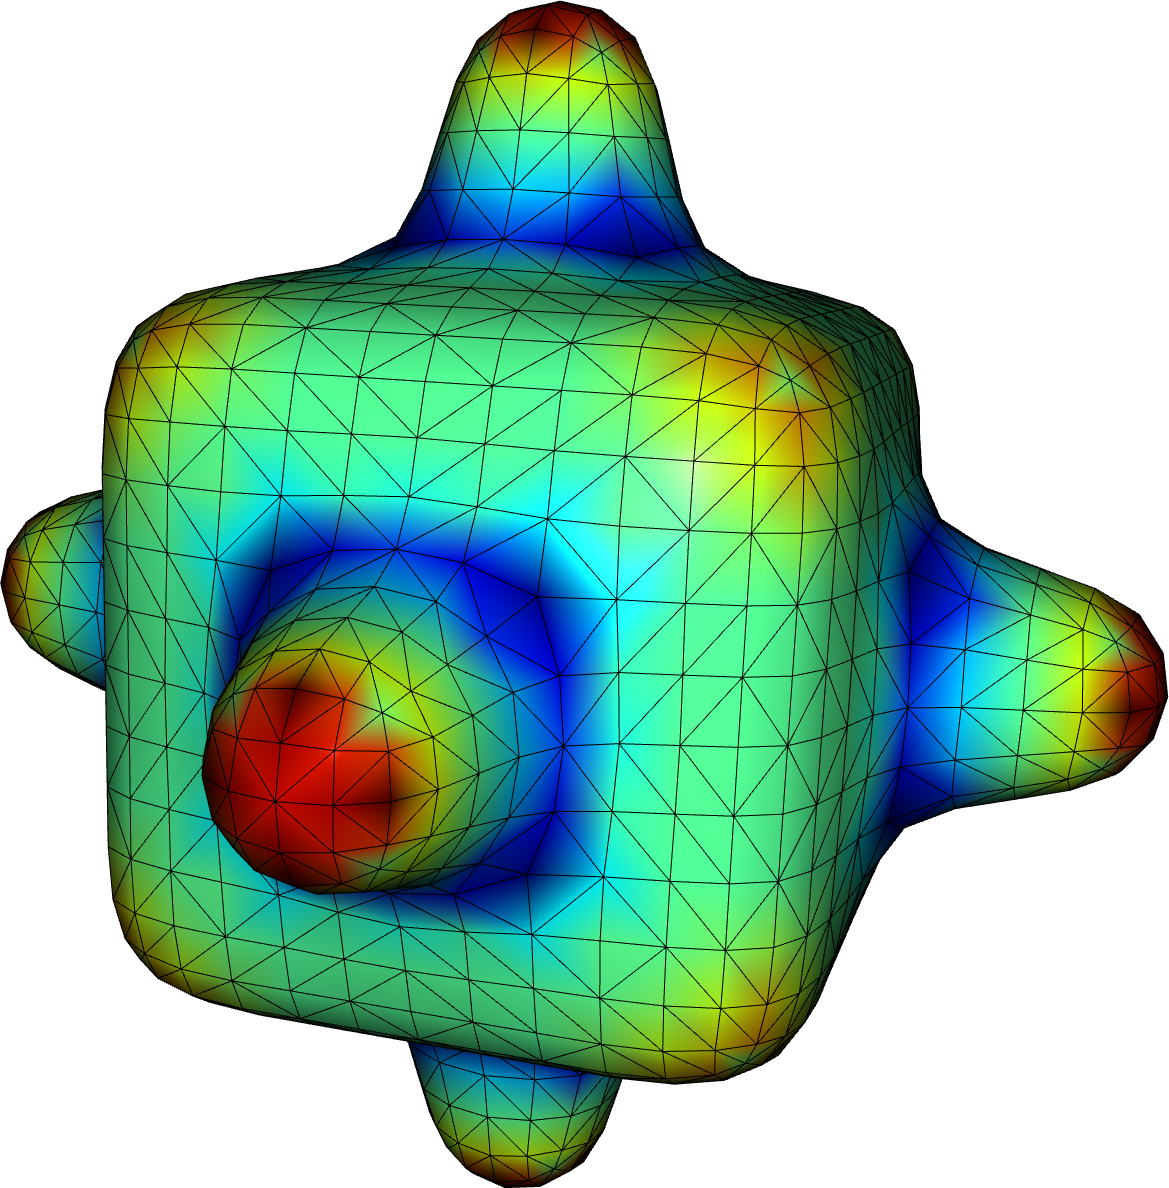
\includegraphics[width=0.3\linewidth]{gauss_curv}}
\hspace{1.5cm}
   \subfloat[Gaussian Curvature]{\label{fig:curv_directions}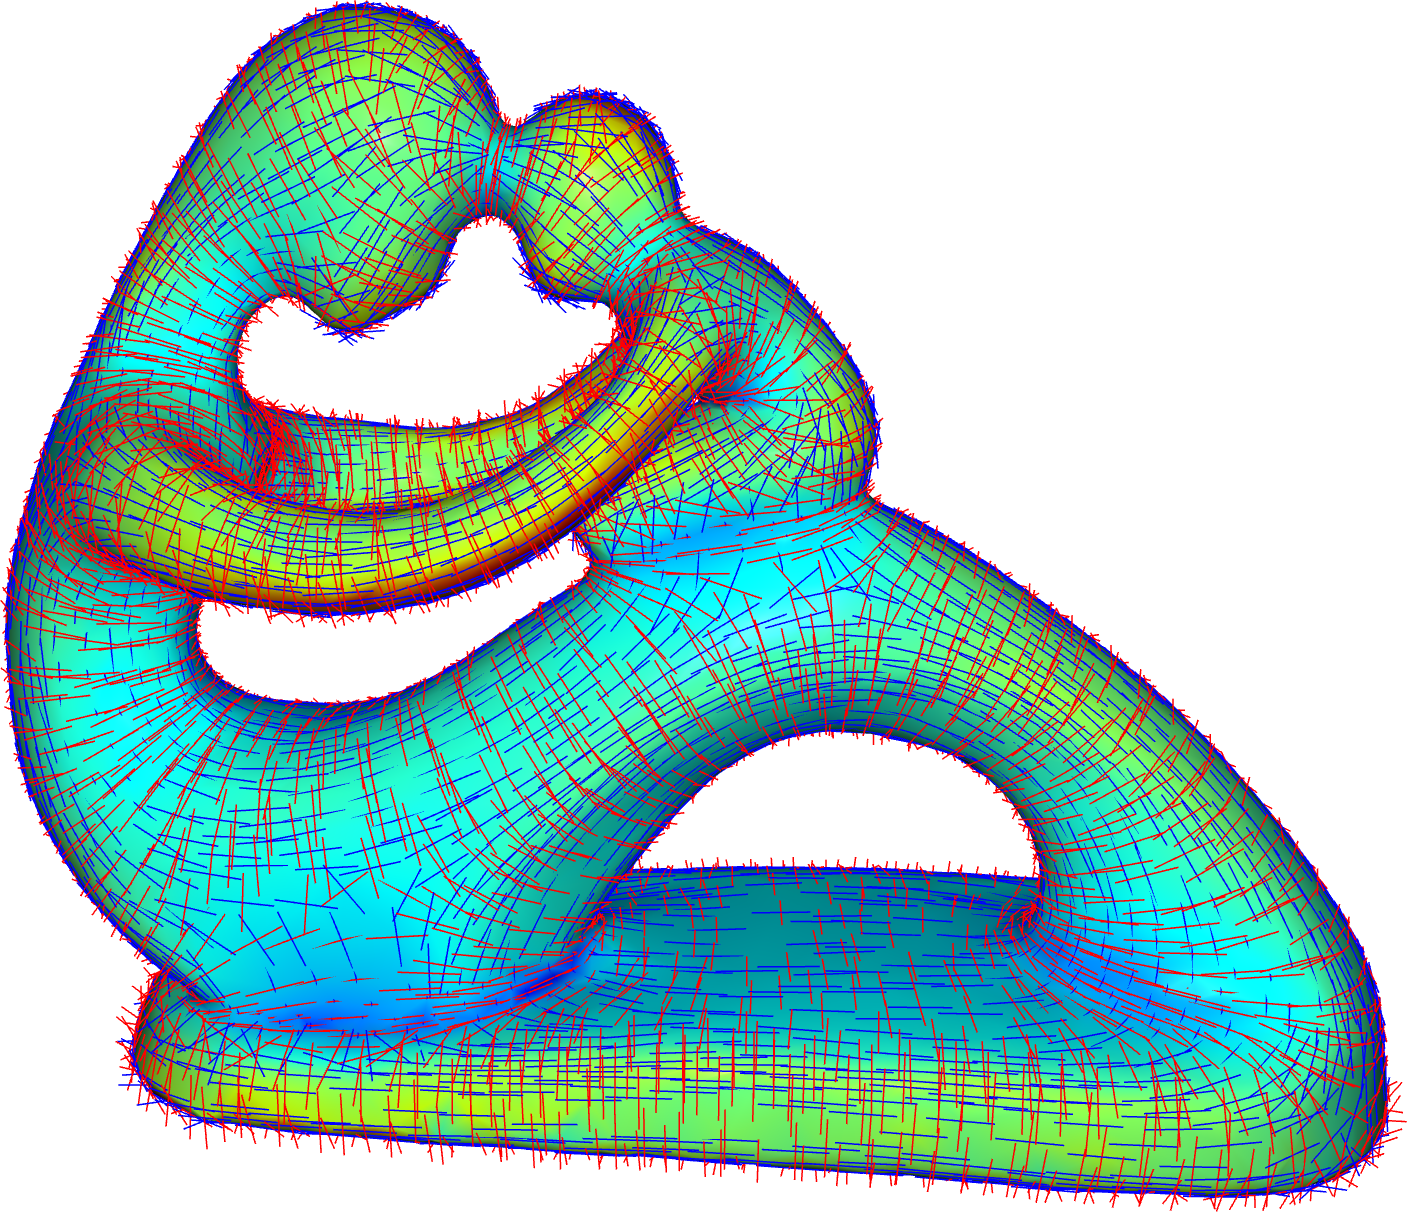
\includegraphics[width=0.3\linewidth]{curv_directions}}
%\hspace{1cm}
   \caption{On the left: Gaussian curvature visualization. On the right,
    mean curvature and principal curvature directions.}
   \label{fig:beetle}
\end{figure}

\emph{Relevant} \texttt{libigl} \emph{functions: }
\texttt{igl::gaussian\_curvature}, \texttt{igl::principal\_curvature},
\texttt{igl::cotmatrix}, \texttt{igl::massmatrix}.

\section{Smoothing with the Laplacian}
\begin{figure}[H]
   \centering
   \subfloat[original]{\label{fig:cow_orig}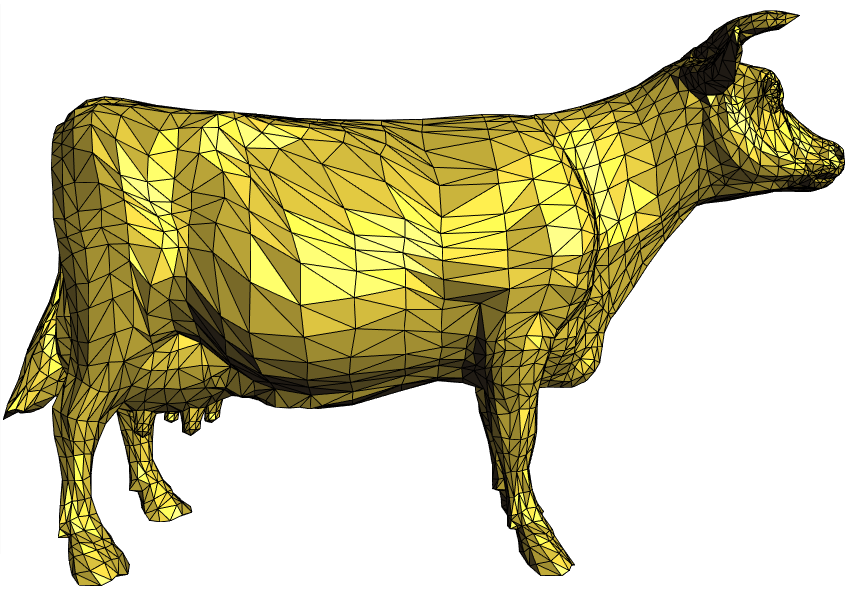
\includegraphics[width=0.29\linewidth]{cow_orig.png}}
\hspace{0.4cm}
   \subfloat[explicit smoothing, $\lambda = 0.01$, 1000 iterations]{\label{fig:cow_explicit}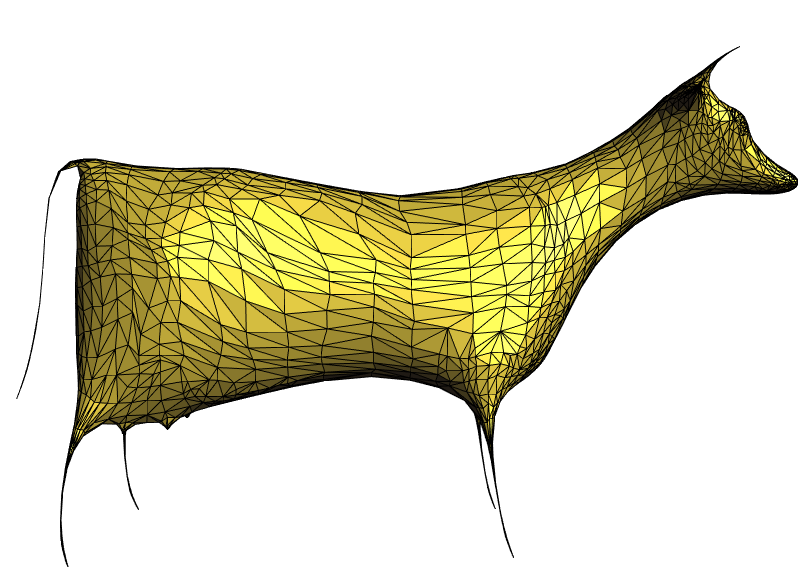
\includegraphics[width=0.32\linewidth]{cow_explicit_l001_iter1000.png}}
\hspace{0.4cm}
   \subfloat[implicit smoothing, $\lambda = 20$, 1 iteration]{\label{fig:cow_implicit}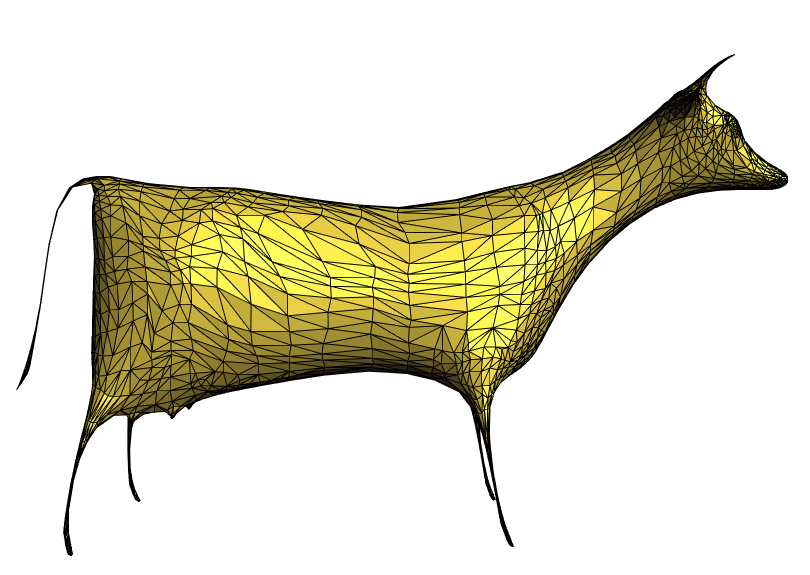
\includegraphics[width=0.32\linewidth]{cow_implicit_l20_iter1.png}}
   \caption{Explicit and implicit smoothing on the \emph{cow} mesh.}
   \label{fig:cow}
\end{figure}
Perform explicit and implicit Laplacian mesh smoothing. Experiment with uniform
and cotangent weights. Before you begin, check out tutorial \# 205, which
implements implicit smoothing.  

\emph{Relevant} \texttt{libigl} \emph{functions: } \texttt{igl::cotmatrix}, \texttt{igl::massmatrix}, \texttt{igl::grad}, \texttt{igl::doublearea}.

\section{Bilateral Smoothing}
Implement bilateral mesh smoothing as described in
\href{http://www.cs.tau.ac.il/~dcor/online_papers/papers/shachar03.pdf}{"Bilateral
Mesh Denoising"} by Fleishman et al.
\end{document}
